\documentclass[9pt,twocolumn,twoside,]{pnas-new}

% Use the lineno option to display guide line numbers if required.
% Note that the use of elements such as single-column equations
% may affect the guide line number alignment.


\usepackage[T1]{fontenc}
\usepackage[utf8]{inputenc}

% tightlist command for lists without linebreak
\providecommand{\tightlist}{%
  \setlength{\itemsep}{0pt}\setlength{\parskip}{0pt}}


% Pandoc citation processing
\newlength{\cslhangindent}
\setlength{\cslhangindent}{1.5em}
\newlength{\csllabelwidth}
\setlength{\csllabelwidth}{3em}
\newlength{\cslentryspacingunit} % times entry-spacing
\setlength{\cslentryspacingunit}{\parskip}
% for Pandoc 2.8 to 2.10.1
\newenvironment{cslreferences}%
  {}%
  {\par}
% For Pandoc 2.11+
\newenvironment{CSLReferences}[2] % #1 hanging-ident, #2 entry spacing
 {% don't indent paragraphs
  \setlength{\parindent}{0pt}
  % turn on hanging indent if param 1 is 1
  \ifodd #1
  \let\oldpar\par
  \def\par{\hangindent=\cslhangindent\oldpar}
  \fi
  % set entry spacing
  \setlength{\parskip}{#2\cslentryspacingunit}
 }%
 {}
\usepackage{calc}
\newcommand{\CSLBlock}[1]{#1\hfill\break}
\newcommand{\CSLLeftMargin}[1]{\parbox[t]{\csllabelwidth}{#1}}
\newcommand{\CSLRightInline}[1]{\parbox[t]{\linewidth - \csllabelwidth}{#1}\break}
\newcommand{\CSLIndent}[1]{\hspace{\cslhangindent}#1}


\templatetype{pnasresearcharticle}  % Choose template

\title{Réseau de coopération des étudiants de BIO500}

\author[a]{Yanick Sageau}
\author[a]{Samuel Beaulac}
\author[a]{Sabrina Leclercq}
\author[a]{Cassangra Godin}

  \affil[a]{Université de Sherbrooke, Département de biologie, Bd de
L'Université, Sherbrooke, Québec, J1K2R1}


% Please give the surname of the lead author for the running footer
\leadauthor{}

% Please add here a significance statement to explain the relevance of your work
\significancestatement{}


\authorcontributions{}



\correspondingauthor{\textsuperscript{} }

% Keywords are not mandatory, but authors are strongly encouraged to provide them. If provided, please include two to five keywords, separated by the pipe symbol, e.g:


\begin{abstract}
Dans le cadre du cours de BIO500, nous avons été invités à faire une
étude comparative concernant les collaborations des étudiants de
biologie et leurs possibles ressemblances à certaines communautés et
réseaux écologiques. Une collecte de données auprès des étudiants et des
analyses faites à partir de R studio ont permis la réalisation de ce
projet. De cette manière, la visualisation de notre réseau de
collaborations entre étudiants a révélé des similarités avec des réseaux
trophiques écologiques. De plus, d'autres liens écologiques ont pu être
observés avec les résultats d'analyse concernant d'autres facteurs qui
influencent les interactions, comme la région d'origine des étudiants et
leur session de début de baccalauréat. En bref, bien que les
interactions entre étudiants en biologie ne soient pas totalement les
mêmes que dans les réseaux trophiques et les communautés écologiques, on
peut y voir certains patrons de ressemblances pouvant aider à expliquer
les interactions sociales des individus.
\end{abstract}

\dates{This manuscript was compiled on \today}
\doi{\url{www.pnas.org/cgi/doi/10.1073/pnas.XXXXXXXXXX}}

\begin{document}

% Optional adjustment to line up main text (after abstract) of first page with line numbers, when using both lineno and twocolumn options.
% You should only change this length when you've finalised the article contents.
\verticaladjustment{-2pt}



\maketitle
\thispagestyle{firststyle}
\ifthenelse{\boolean{shortarticle}}{\ifthenelse{\boolean{singlecolumn}}{\abscontentformatted}{\abscontent}}{}

% If your first paragraph (i.e. with the \dropcap) contains a list environment (quote, quotation, theorem, definition, enumerate, itemize...), the line after the list may have some extra indentation. If this is the case, add \parshape=0 to the end of the list environment.

\acknow{}

\hypertarget{introduction}{%
\subsection{Introduction}\label{introduction}}

En écologie, les réseaux d'interactions biotiques et abiotiques sont
d'intérêt pour mieux comprendre les organismes qui en font partie. Ces
réseaux sont souvent utilisés pour plusieurs types d'analyses et de
modèles d'assemblage, comme pour les réseaux trophiques (1). D'autres
types de réseaux sont aussi connus, comme des réseaux internet et des
réseaux de groupes sociaux (interactions sociales entre humains, un peu
comme les animaux!). Ce projet s'intéresse à analyser les propriétés des
réseaux d'interactions entre les élèves de la classe et d'autres
étudiants dans le département de biologie à l'Université de Sherbrooke
en essayant de répondre à certaines questions de recherches de nature
écologique. Est-ce que les propriétés du réseau de collaboration entre
étudiants de biologie diffèrent de celles des réseaux écologiques?
Est-ce que les étudiants qui proviennent de la même région
administrative collaborent plus ensemble? Est-ce que la session de début
de baccalauréat influence les interactions entre étudiants? Afin de
répondre à ces questions, le travail qui suit comportera la description
des méthodes utilisées, la présentation des résultats, l'analyse de
ceux-ci dans la discussion et une brève conclusion.

\hypertarget{muxe9thode}{%
\subsection{Méthode}\label{muxe9thode}}

La première étape du projet était la collecte de données des étudiants
dans la classe via trois fichiers Excel sur les collaborations entre
étudiants, les informations sur les cours où il y a eu collaboration et
les informations de l'étudiant (nom, région administrative d'origine,
session de début de baccalauréat et le nom du programme d'étude).

Une fois ces informations fournies par les étudiants, les données ont
été comptabilisées en créant une base de données regroupant les données
de tous les étudiants du cours. À noter que toutes les étapes, de la
création de la base de données jusqu'aux résultats, ont été effectuées à
l'aide de R Studio.

Après avoir créé la base de données, un nettoyage a été nécessaire afin
de retirer les colonnes et les rangées vides, fusionner les rangées des
documents, supprimer les documents individuels, supprimer les doublons,
corriger les noms des étudiants ou des colonnes écris incorrectement,
changer les cases vides pour NA, changer les rangées vrai/faux pour
TRUE/FALSE et mettre les données dans l'ordre.

Une fois les données nettoyées, des tableaux «sql» ont été créés pour
ensuite y injecter nos données et faire les requêtes et analyses.

À partir des tables «sql», diverses requêtes concernant nos questions de
recherches ont pu être effectuées et avec ces résultats, les figures ont
été créées.

Les étapes d'analyse ont été divisées en différentes étapes targets pour
établir un «pipeline» et afin d'optimiser la reproductibilité du
travail.

\hypertarget{ruxe9sultats}{%
\subsection{Résultats}\label{ruxe9sultats}}

En créant une matrice avec les interactions/collaborations présentes et
absentes entre les étudiants, un graphique en toile a été généré (Figure
1 -\textgreater{} réseau interactions). Cette figure permet de
visualiser le réseau d'interactions des étudiants en biologie.

\begin{figure}
\centering
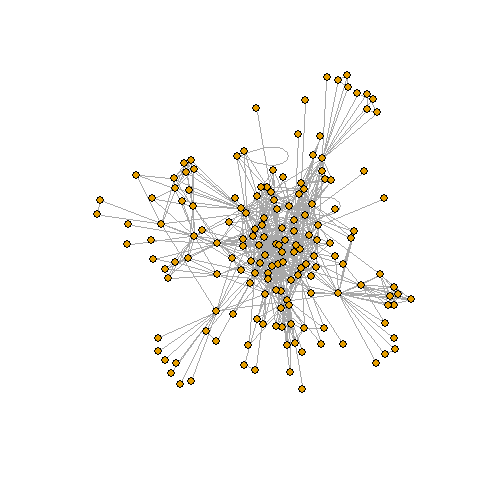
\includegraphics[width=0.4\textwidth,height=0.3\textheight]{"../interactions.png"}
\caption{Réseau d'intéractions entre les étudiants de BOT500 et leurs
collaborateurs dans leurs projets d'équipe}
\end{figure}

Afin d'obtenir les résultats pour les interactions/collaborations par
rapport à la région administrative d'origine, un test de Mantel a été
effectué à partir de matrices. Dans la Figure 2 (interactions-régions),
l'histogramme montre la différence entre les interactions des étudiants
provenant de la même région et ceux provenant de régions différentes. Un
graphique n'a pas été produit pour ce paramètre, puisque la corrélation
n'était pas significative (p-value = 0,147), mais l'histogramme permet
quand même d'interpréter les résultats.

\begin{figure}
\centering
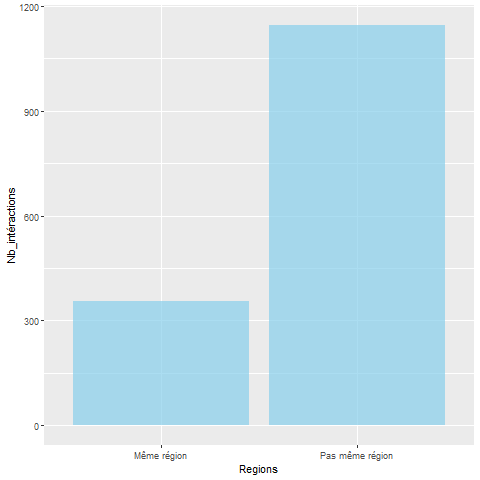
\includegraphics[width=0.4\textwidth,height=0.3\textheight]{"../region.png"}
\caption{Quantité d'interactions si la région de provenance est
identique ou non}
\end{figure}

La Figure 4 (interaction session graphique) montre la relation entre les
matrices de distances des interactions par rapport à la session de début
de baccalauréat.

\begin{figure}
\centering
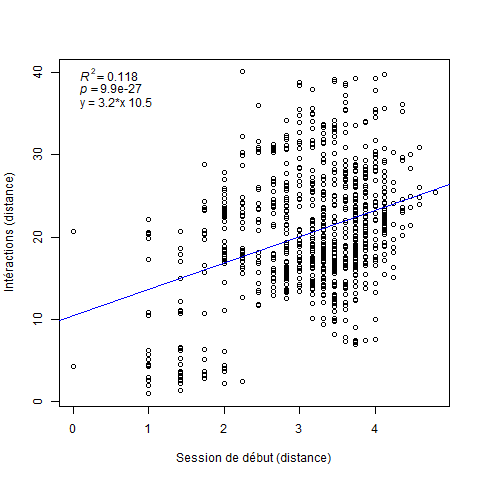
\includegraphics[width=0.4\textwidth,height=0.3\textheight]{"../plot.png"}
\caption{Relation des interactions entre étudiants par rapport à leur
année de début de baccalauréat}
\end{figure}

Les figures concernant les interactions/collaborations et la session de
début de baccalauréat ont aussi été faites avec un test de Mantel, mais
avec des matrices de distance. La Figure 3 (interaction session
bar-plot) montre la différence entre les interactions des étudiants qui
ont commencé leur baccalauréat à la même session et les interactions de
ceux qui n'ont pas commencé à la même session.

\begin{figure}
\centering
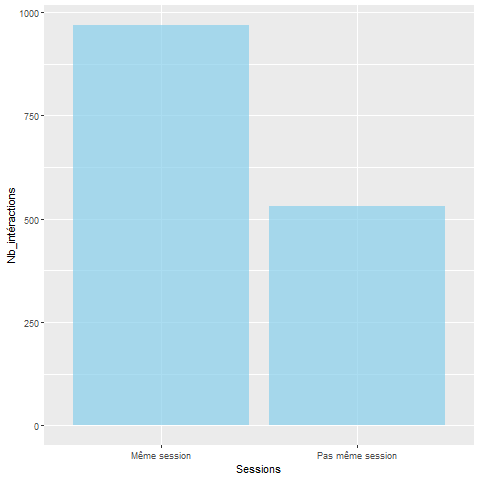
\includegraphics[width=0.4\textwidth,height=0.3\textheight]{"../annee.png"}
\caption{Relation des interactions entre étudiants par rapport à leur
année de début de baccalauréat}
\end{figure}

\hypertarget{discussion}{%
\subsection{Discussion}\label{discussion}}

La question principale du projet était de voir si le réseau de
collaboration entre étudiants de biologie était similaire à un réseau
écologique. La meilleure façon de répondre à cette question est de
comparer notre réseau à d'autres réseaux de nature écologique. Si on
compare notre réseau à un réseau trophique (food web) (Figure 5) (2) et
à un réseau de dépendance dans un réseau trophique (Figure 6) (3), on
observe certaines ressemblances avec le réseau étudiant (Figure 1).

\begin{figure}
\centering
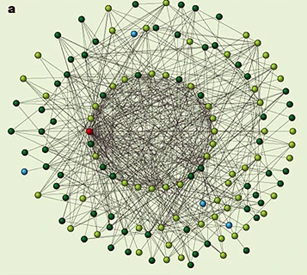
\includegraphics[width=0.4\textwidth,height=0.3\textheight]{"../inter_gros.png"}
\caption{Food web obtenu dans l'article (2)}
\end{figure}

\begin{figure}
\centering
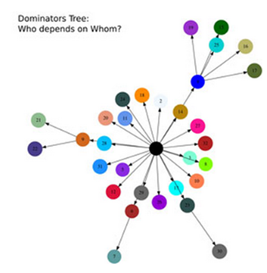
\includegraphics[width=0.4\textwidth,height=0.3\textheight]{"../inter_petit.png"}
\caption{Réseau de dépendance dans un réseau trophique obtenu dans
l'article (3)}
\end{figure}

On remarque que dans tous les réseaux, il semble y avoir un agrégat
d'interactions au centre du réseau, et vers l'extérieur, de plus petits
groupes isolés. Dans un réseau trophique, les noeuds vers les extrémités
sont souvent représentés par les prédateurs en haut de la chaîne
alimentaire et ceux se dirigeant vers le centre sont des prédateurs de
plus bas niveau, des herbivores, les producteurs primaires, des
détritivores, etc\ldots{} (2). Il est donc normal qu'il y ait plus
d'interactions au centre du réseau. Évidemment, les interactions dans
ces réseaux trophiques ne sont pas les mêmes que dans notre réseau de
collaboration entre étudiants et il est donc difficile de les comparer
(4), mais il est tout de même possible d'y observer des similitudes. On
pourrait comparer les prédateurs des réseaux trophiques avec les
personnes les plus riches dans un réseau social humain (2). Aussi, des
ressemblances ont été observées concernant les réseaux d'interactions
entre animaux et ceux entre humains pour le transfert de maladie (4).

Dans la Figure 2, on observe qu'il y environ 3 fois plus d'interactions
entre les étudiants qui ne proviennent pas de même région et ceux qui
proviennent de la même région. Cela peut sembler contre-intuitif à
première vue, mais on observe des phénomènes semblables en écologie par
la dispersion. En effet, la migration peut être bénéfique dans le cas
d'un déplacement vers un nouvel environnement favorable (5), mais elle
favorise aussi les interactions entre des individus différents qui ne
proviennent pas des mêmes populations (6). Ces interactions sont
avantageuses pour augmenter la variabilité génétique, donc les
organismes ont souvent tendance à plus interagir avec des individus
différents pour augmenter la diversité du flux génétique (6). Dans le
cas de nos collaborations, comme en écologie, il pourrait être
avantageux pour les étudiants d'interagir avec des personnes différentes
de celles qu'ils connaissent (ou de même provenance) pour élargir et
diversifier leurs interactions et leurs perspectives sur divers sujets,
ce qui pourrait être utile dans l'élaboration d'un travail scolaire par
exemple.

D'autres facteurs externes influencent les interactions dans les réseaux
trophiques et dans notre réseau de collaborations, comme la distance et
le temps d'arrivée à un endroit. D'après (1), il y a trois aspects
interreliés qui peuvent influencer l'assemblage d'espèces ; le taux
d'assemblage (le temps entre deux colonisations), la variabilité des
taux d'assemblage et l'agrégation (puisque les espèces peuvent arriver
en groupe par chance ou par d'autres phénomènes aléatoires). On pourrait
appliquer ceci à nos résultats des collaborations des étudiants, par
exemple, le temps entre colonisations peut faire référence à la session
de début du baccalauréat. En effet, il y avait corrélation significative
entre la session de début d'étude et les collaborations (Figure 4)
puisque le p-value était de 9.9e-27. Aussi, dans la Figure 3, on peut
observer qu'il y a presque deux fois plus de collaborations entre les
étudiants qui ont commencé à la même session par rapport à ceux qui ont
commencé à des sessions différentes. Cela pourrait aussi être comparé au
principe de spéciation allopatrique chez les animaux (7, 8), puisque les
sessions de départ différentes agiraient comme une barrière (ici, pas
une barrière physique) pour les interactions entre ces étudiants,
puisque les chances de contact et d'échanges sont réduites par cette
barrière.

\hypertarget{conclusion}{%
\subsection{Conclusion}\label{conclusion}}

En conclusion, en comparant les résultats obtenus avec notre réseau de
collaborations entre étudiants en biologie avec les théories
écologiques, on peut observer plusieurs similarités entre les deux, tant
dans la visualisation du réseau (comparé avec un réseau trophique
écologique), que dans les autres aspects influençant les interactions
des étudiants comme la région d'origine et la session de début d'étude.
Dans la perspective d'un futur projet, il serait intéressant de faire le
même type d'étude comparative, mais avec plusieurs départements de
l'Université pour déterminer si les réseaux d'interactions sont
semblables aux réseaux écologiques.

\hypertarget{refs}{}
\begin{CSLReferences}{0}{0}
\leavevmode\vadjust pre{\hypertarget{ref-gounand2015interactions}{}}%
\CSLLeftMargin{1. }%
\CSLRightInline{Gounand I (2015) Interactions multi-échelles entre
ressources abiotiques, réseaux trophiques et propriétés des écosystèmes:
Nouveaux jalons théoriques pour une écologie intégrative. PhD thesis
(Université du Québec à Rimouski).}

\leavevmode\vadjust pre{\hypertarget{ref-montoya2006ecological}{}}%
\CSLLeftMargin{2. }%
\CSLRightInline{Montoya JM, Pimm SL, Solé RV (2006) Ecological networks
and their fragility. \emph{Nature} 442(7100):259--264.}

\leavevmode\vadjust pre{\hypertarget{ref-etemad2014spirograph}{}}%
\CSLLeftMargin{3. }%
\CSLRightInline{Etemad K, Carpendale S, Samavati F (2014) Spirograph
inspired visualization of ecological networks. \emph{Proceedings of the
Workshop on Computational Aesthetics}, pp 81--91.}

\leavevmode\vadjust pre{\hypertarget{ref-perkins2009comparison}{}}%
\CSLLeftMargin{4. }%
\CSLRightInline{Perkins SE, Cagnacci F, Stradiotto A, Arnoldi D, Hudson
PJ (2009) Comparison of social networks derived from ecological data:
Implications for inferring infectious disease dynamics. \emph{Journal of
Animal Ecology} 78(5):1015--1022.}

\leavevmode\vadjust pre{\hypertarget{ref-gibson2003go}{}}%
\CSLLeftMargin{5. }%
\CSLRightInline{Gibson RN (2003) Go with the flow: Tidal migration in
marine animals. \emph{Migrations and Dispersal of Marine Organisms:
Proceedings of the 37 Th European Marine Biology Symposium Held in
Reykjavík, Iceland, 5--9 August 2002} (Springer), pp 153--161.}

\leavevmode\vadjust pre{\hypertarget{ref-carvalho1993evolutionary}{}}%
\CSLLeftMargin{6. }%
\CSLRightInline{Carvalho G (1993) Evolutionary aspects of fish
distribution: Genetic variability and adaptation. \emph{Journal of Fish
Biology} 43:53--73.}

\leavevmode\vadjust pre{\hypertarget{ref-brooker2007modelling}{}}%
\CSLLeftMargin{7. }%
\CSLRightInline{Brooker RW, Travis JM, Clark EJ, Dytham C (2007)
Modelling species' range shifts in a changing climate: The impacts of
biotic interactions, dispersal distance and the rate of climate change.
\emph{Journal of theoretical biology} 245(1):59--65.}

\leavevmode\vadjust pre{\hypertarget{ref-lande1980genetic}{}}%
\CSLLeftMargin{8. }%
\CSLRightInline{Lande R (1980) Genetic variation and phenotypic
evolution during allopatric speciation. \emph{The American Naturalist}
116(4):463--479.}

\end{CSLReferences}



% Bibliography
% \bibliography{pnas-sample}

\end{document}
